\newpage
\subsection{Zusammenfassung}\label{implementierung_zusammenfassung}

Der vollständige Workflow der CI/CD Pipeline wird im untenstehenden Bild dargestellt.

\begin{figure}[htb]
    \centering
    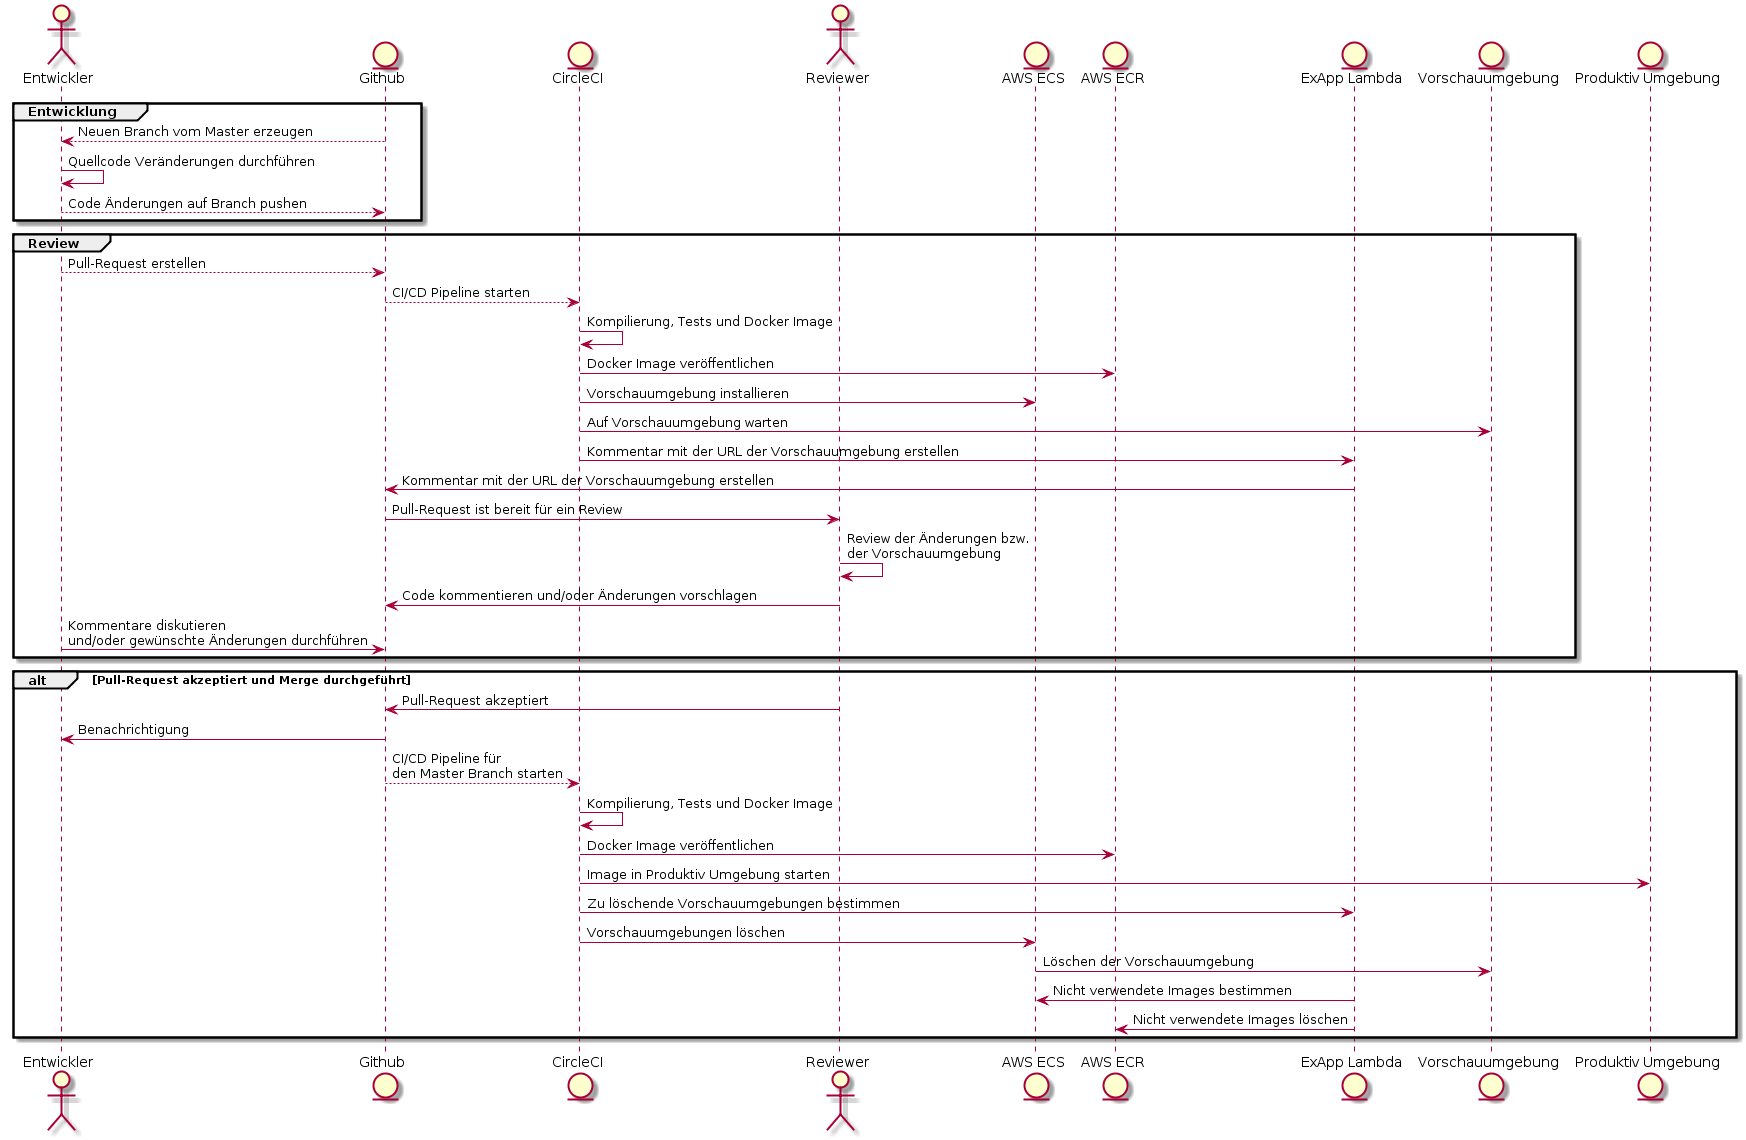
\includegraphics[width=1.0\textwidth]{images/workflow.png}
    \caption[Circle CI Workflow]{Circle CI Workflow}
    \label{fig:circle_ci_workflow}
\end{figure}

Die implementiere CI/CD-Pipeline ermöglicht eine Self Service Infrastruktur.
Entwickler können durch Veränderungen an den Terraform Skripten die Infrastruktur anpassen.
Die Pipeline führt diese Änderungen aus und ermöglicht durch das Bereitstellen einer Vorschauumgebung effiziente Review Prozesse. \\

Der Entwickler muss nur einen Pull Request öffnen, um die Automatisierung zu starten.
Nach Abschluss aller Tests und der testweisen Veröffentlichung kann ein Review durchgeführt werden.
Der Reviewer kann die Veränderungen direkt in der Vorschauumgebung ausprobieren. \\

Wird ein Pull-Request akzeptiert, genügt ein Knopfdruck um den Pull-Request zu akzeptieren und damit den neuen Code in die Produktion zu überführen.
Im Fehlerfall kann eine Änderung in Git wieder rückgängig gemacht werden und die CI/CD Pipeline wird die vorherige Version wiederherstellen.

